In recent decades, cognitive science has deepened our understanding of the mechanisms that subserve skill learning and has begun to spark ideas on how to achieve better learning by leveraging these mechanisms more effectively \parencite{wolpert_principles_2011, makino_circuit_2016, spampinato_multiple_2021, krakauer_motor_2019, haith_model-based_2013, huang_rethinking_2011, shmuelof_are_2011, doya_complementary_2000}. Thus far, most studies have focused on simple, laboratory-based tasks \parencite{krakauer_motor_2019, du_relationship_2022, yarrow_inside_2009}, raising concerns about their applicability to real-world learning in areas such as sports, education, or rehabilitation. Therefore, there is a pressing need for studies with greater ecological validity, where learning tasks are not trivial exercises but instead improve important life functions or skills that learners genuinely care about \parencite{spampinato_multiple_2021, du_relationship_2022}. The overarching goal of this doctoral thesis was to bridge this gap between simple tasks and real-world skill learning with skilled performers using alpine skiing as a domain to test these theories. To achieve this goal, this doctoral thesis adopted a crossdisciplinary research approach involving mechanics and psychology. From a mechanical perspective, we asked what is the most effective strategies for skiing faster on flat slopes (research aim 1) and the kinematic signatures that make one of these strategies so effective (research aim 2). From a psychological perspective, we asked whether better learning effects could be achieved by applying learning theories from cognitive science to create learning problems (research aim 3) and better utilize teaching signals (research aim 4).  

First, we found that skiers on average achieved the fastest race times using the "extend with rock skis forward" strategy, which aligns with our expectations based on theory and quantitative field observations. This suggests that this strategy is powerful and can improve the performance of skiers on flats in slalom. However, its effect was only marginally better than that of the "extend" strategy, which is simpler and nearly as effective on its own. Based on these results, we recommend that skiers choose either of these two strategies to enhance their performance on flat sections in slalom. These findings expand upon previous ski research and provide experimental evidence for effective strategies to ski fast on flats in slalom.

Second, we also found that a training intervention focusing on the "extend" strategy left a remarkable kinematic signature on the skiers. After the intervention, skiers exhibited a more wave-like speed profile. That is, they increased their speed after passing through a gate, which continued to rise until they were approximately midway between two gates. Then, their speed decreased until the next gate, before increasing again. Additionally, we observed a trend where skiers took longer paths between gates, yet their race times improved. Together, these kinematic signatures closely resemble the predictions from Lind and Sander's model of pumping to increase velocity. A limitation of our data is that we do not know the specific movements the skiers made, preventing us from testing the model's predictions accurately. Future research should employ motion capture technology to achieve the necessary data quality for such investigations.

Shifting focus toward the testing of learning theories to improve skill learning, we did not find evidence that the skiers learned better by increasing the frequency at which they were exposed to new learning problems (that is, interleaved practice). This finding aligns with prior research that has similarly failed to observe a contextual interference effect in real-world tasks or more complex learning tasks  \parencite{brady_theoretical_1998, barreiros_contextual_2007, wulf_principles_2002}. Based on the results of this study and these previous findings, it may not be worthwhile to expend effort in creating multiple different slalom courses, at least concerning performance outcomes. Nonetheless, we should not dismiss the possibility that exposing skiers to rapid changes in course could influence other cognitive mechanisms. It is also plausible that the benefit of frequent course changes lies in preventing habits \parencite{du_relationship_2022}, whereby skiers settle on a fixed solution and become insensitive to adapting to different situations. If so, simply changing courses sufficiently often might be adequate to avoid these habits. To better understand this phenomenon, an alternative experimental design is crucial. One approach could involve training hairpins, with one learning group practising only one hairpin while another group practising multiple hairpins.

Finally, we found that learning strategies and their values through reinforcement learning provided a more effective teaching signal than conventional instruction-based coaching. Interestingly, the reinforcement learning group also performed better than the supervised (target skill) learning group, which was intended to represent the upper limit of performance achievable through optimal strategy choices. The effect size was substantial enough to potentially impact skiers' world rankings based on their FIS points. Our hypothesis that the difference between groups was due to better strategy selection on the single best strategy was not supported. The reinforcement learning group did not begin with, nor develop, a greater probability of choosing the theoretically optimal strategy or the individual skier's estimated best strategy compared to the supervised (free choice) learning group. Instead, we found that the expected loss in time for skiers who made suboptimal choices (i.e., cost or expected regret) during retention was lower in the reinforcement learning group than in the supervised (free choice) learning group. This suggests that the reinforcement learning group learned to select strategies that offered comparable outcomes and avoided those with a risk of significantly worse performance. One possibility is that the reinforcement learning group discovered that the "extend" strategy alone provided nearly full benefits and chose this strategy for its simplicity over "extend with rock skis forward." See Paper \RNum{3} for complete results and discussion. 

The findings from this study suggest that reinforcement learning can serve as an effective teaching signal for selecting optimal strategies and performance. The key question is how coaches or teachers can apply this knowledge in practice. One approach is to replicate the strategies developed for the study and teach skiers to use them. However, the application can be simplified or made more advanced depending on the skill level or experience of the skiers. For less skilled skiers, learning can occur by having them ski high and low in tuck positions to observe the impact of air drag on their times, or by creating multiple line choices around a gate and allowing skiers to experiment with them. For more skilled skiers, a narrower set of strategies that are expected to produce smaller yet meaningful and interpretable differences can be developed. The general principle to make reinforcement learning effective is to design strategies that challenge expectations, ideally with one strategy outperforming the expected outcomes. Once skiers have established a solid understanding of the value of different strategies, it may become less useful to continue gaining experience with those strategies. At this point, coaches can either develop new sets of strategies or shift their learning strategy, such as focusing on refining the execution of the strategies. 

Beyond addressing the four key questions, the thesis revealed broader insights crucial for evaluating the research in this thesis and for advancing future studies on elite alpine skiers. The first of these broader insights was the method of quantifying performance in alpine skiing. This has been a widely debated issue, with scientists proposing various measures such as energy mechanics \parencite{supej_differential_2008, supej_how_2010, supej_mechanical_2011} , differences in mechanical energy divided by time, section times \parencite{supej_relations_2006}, lateral skidding of skis \parencite{kirby_development_2009}, and time loss per elevation difference and distance travelled per elevation difference \parencite{federolf_quantifying_2012}. Throughout this thesis, I have quantified performance in terms of race time to operate on the same scale as skiers and coaches do since this is the conventional way to quantify performance in skiing. Men jeg har kvantifisert på two ulike måter: in Papers \RNum{1} and \RNum{2}, I have expressed race time as the difference from the time when the skier skied the section straight down (straight gliding), whereas, in Paper \RNum{3}, I used the raw race time to quantify performance.

To initiate the discussion on the insights gained from using race times to quantify performance, I have conducted a Bayesian multilevel growth model on all the skiers' times as they skied straight down the section in all sessions presented in Paper  \RNum{3}. From this analysis, I found that the straight gliding times for all ski groups (A, B, C, and D) increased steadily from the first session (baseline) to the last session (transfer). Fig. \ref{fig:straightgliding} shows these trends. Although I cannot entirely rule out any explanation for why the straight gliding times of the ski groups increased uniformly, I am confident that differences in the length of the course section are not the main explanation. This is because we used a measuring tape during the course setting, and there was a tight cluster of boreholes at the finish line, with only a few centimeters of difference. I also do not believe that changes in the skiers' starting procedures or execution of straight gliding are the main reasons. This is because the skiers were diligent and interested in performing this task as well as possible. I believe the best explanation involves the snow conditions and how we prepared them. Specifically, when grooming snow with a machine, grooves are left in the snow that becomes hard if it is watered and allowed to freeze. These hard grooves are fast to ski on because only a small part of the ski is in contact with the snow surface. As skiers complete more runs and coaches slide through the course, these snow grooves wear away, creating a smooth, hard base without grooves. When skiers descend on this groom-free base, a larger part of the ski’s contact surface touches the snow, which increases ski–snow friction and slows the skiers down.


\begin{figure}
    \centering
    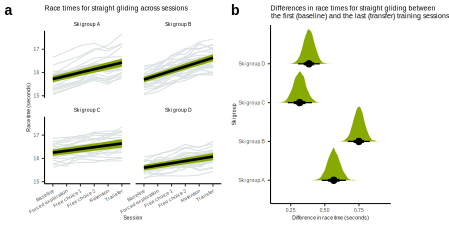
\includegraphics[width=1\linewidth]{figure/figure_methodological_straightgliding.pdf}
    \caption[Straight gliding times across the sessions]{Straight gliding times across the sessions.\textbf{ a.} Expected change in straight gliding times across the training sessions for groups of ski teams that were tested. \textbf{b.} Expected change in means from baseline to transfer for the groups of ski teams that were tested together. The black lines denote the expected means or differences in means, with the shaded area representing the 95\% credible interval (CI). Each gray line represents one straight gliding run by a skier.}
    \label{fig:straightgliding}
\end{figure}


What consequences does this have for the interpretation of results in this thesis, and how can we address these challenges in future studies in the best possible way? First, one challenge this creates is the need to exercise caution in interpreting 'true' learning from the estimated change in race times. From Fig. \ref{fig:rlstudy_racetime} from Study \RNum{2}, we find that the skiers improved their race times greatly over the sessions despite the increased straight gliding times. Therefore, the 'true' improvement is likely better than estimated. A less conservative and perhaps better way to express skiers' 'true' learning is to use the difference in straight gliding times for each session to account for variations in the snow surface. This is the performance measure we used in Study \RNum{1}. However, although this measure may better capture skiers' learning, we do not know whether it underestimates or overestimates learning. Another problem is that straight gliding in itself is a random variable that introduces variation and could add noise to the measurement. In Study \RNum{2}, we had to move away from this measure because the straight gliding lane crossed many holes from the previous courses. Due to these challenges, it is difficult to determine the actual improvement of skiers. Scientists therefore face two choices: either use raw race times, which is likely a conservative method that underestimates the real improvement, or express time as the difference in straight gliding, which may better account for variations in the surface and therefore express progress more accurately. The cost of the latter approach is that it underestimates or overestimates performance and could increase noise. Another solution is to downplay the focus on change and determine whether the learning groups differ on the postmeasure if their performance is equal at baseline, corresponding to the logic of an ANCOVA \parencite{maxwell_designing_2017}. If we have a design where skiers have undergone tests simultaneously, we can estimate this group difference, indirectly avoiding the question of change. Therefore, we used ANCOVA and raw race data in Study \RNum{2}.

One potential way to improve estimates in future research is to add more levels of skigroups by testing more skiteams. This would allow the groups to have varying effects of the treatment and could achieve better estimates through partial pooling \parencite{mcelreath_statistical_2018, judd_experiments_2017, judd_treating_2012, barr_learning_2021}. We attempted to run this model, but it did not converge due to having too few levels. It might have been better to divide the ski groups into smaller subgroups that were tested at different times. However, it must be emphasized that conducting studies such as ours is very difficult and time-consuming. Consequently, this may not be a feasible approach. Another approach is to skid extensively to eliminate the grooms before testing.

The second additional key insight gained from this thesis is the challenge of determining the smallest effect size of interest (SESOI) in alpine skiing, as the premises for setting such a benchmark are sensitive to variations in external conditions and can change rapidly. In psychological science, it is advised that researchers follow up statistically nonsignificant studies from null-hypothesis significance tests with equivalence testing to better falsify predictions \parencite{lakens_equivalence_2018}. An equivalence test can help in this respect by allowing researchers to determine if the effect is smaller than the SESOI that marks the upper and lowest effect size where the effect size is worth considering. In Paper III, we set the SESOI to a 0.3-second difference in the retention between learning groups. We used this benchmark to simulate data and statistical power for scenarios with 80, 100, and 120 participants. The SESOI was based on our knowledge of alpine skiing and discussions with coaches, but it was intended for a 50-meter longer course and more training sessions than we ultimately ended up using due to practical considerations. We found that the estimated differences between the learning groups were smaller than this benchmark but were statistically significant. It is possible that this SESOI was set too high, but it was still close to the effects we would have been interested in if we had the same conditions as in Study \RNum{1}. In the results and discussion section and in Paper \RNum{3}, we have discussed the potential implications of this estimated effect size. Here, I try to reflect more broadly on the difficulty of setting appropriate SESOIs for alpine skiing research.

In principle, determining SESOI in sports such as alpine skiing should be straightforward due to the quantifiable nature of the sport and the common practice of measuring time differences between skiers. But even in this measurable context, setting such a benchmark proved challenging. One of the main challenges in determining SESOIs for studying differences between learning groups in alpine skiing environments is that raw effects are influenced by external factors such as snow conditions, the length of the slalom course, and the experimental procedures. For instance, a 0.3-second difference between learning groups is less significant if snow conditions are poor and there is greater variability among skiers than if the snow is hard and even. Similarly, a 0.3-second difference is less meaningful for a full-scale 45-second slalom course than for a short 15-second course. The number of training sessions and whether skiers test together or individually, which can introduce treatment diffusion, also impact the significance of this difference. Some of these factors can be predetermined before data collection, while others are dynamic and depend on external and uncontrollable conditions. Together, these variables complicate the determination of the smallest effect size of interest that is valid in all situations. 

An alternative, and perhaps better, solution would have been to develop multiple scenarios for such field experiments and determine the SESOI for each scenario rather than relying on a single scenario. This approach ensures that the SESOI is valid for the conducted experiment. With such an approach, researchers could conduct cost‒benefit analysis \parencite{anvari_using_2021} with coaches and/or athletes to determine the smallest effect size of interest for each scenario. Additionally, involving a large sample in this process could provide a more robust foundation for the SESOI. This method would likely offer a more reliable solution than basing everything on a single situation and unsystematic discussions with coaches, as we did not in Paper \RNum{3}. Future research should at least consider this idea. 

Finally, I would like to evaluate the interdisciplinary approach grounded in mechanics and psychology to study skill learning in skilled and elite athletes. To begin, I would like to argue that from a purely performance-based perspective, this interdisciplinary approach has been successful because the skiers greatly improved their performance by learning these movement strategies. Notably, some skiers improved their race times by more than two seconds, even from an already high skill level. In many cases, these strategies provided a pivotal "aha" moment for many skiers, who then pushed the execution further upon realizing their potential. And in some cases, the changes in execution were so pronounced that the skiers' coaches had difficulty recognizing them. These observations show, in line with previous studies \parencite{ericsson_exceptional_1982, chase_skill_1982, grayshort, grayloooooong}, that continued skill improvement is possible even for highly skilled athletes if better strategies are found. Therefore, using mechanics to develop and learn the effects of strategies to improve performance was a successful approach. However, employing mechanics to develop performance improvement strategies had another positive side effect: it helped recruit skiers for the experiments. As news spread within the skiing community that our research not only contributed to academic knowledge but also improved the performance of skiers, we observed a surge in interest in participating in the study. In total, 186 skilled alpine skiers from Norway and Sweden were tested, including those who served as pilot participants. All these ski teams covered their own travel and accommodation expenses, underscoring the commitment and enthusiasm for the project within the sports community.

The interdisciplinary approach was not entirely without challenges, however. One issue with using mechanical principles to develop strategies is the inherent uncertainty regarding their impact on athletes' performance. In sports such as alpine skiing, numerous factors influence performance, and a strategy that seems mechanically sound might not be effective in practice. This could lead athletes to train inefficient strategies. This was a potential risk with the "extend with rock skis forward" strategy in the supervised (target skill) learning group from Study II. Fortunately, this strategy yielded the best results on average in our case. One crucial strategy to avoid this pitfall is to secure validation from expert coaches before conducting the study. In both learning studies of this thesis, I held several meetings with coaches from the Norwegian alpine skiing team to discuss the strategies to ensure that the strategies would produce the desired effects. Although this approach is not guaranteed to be successful, it can be a critical factor in achieving effective outcomes. Overall, the interdisciplinary approach has proven valuable for studying skill acquisition in elite athletes. Many researchers are now advocating for using more complex and naturalistic tasks to study skill learning \parencite{haar_motor_2020, tsay_bridging_2024, du_relationship_2022, ingram_naturalistic_2011}. However, merely increasing the complexity of tasks is by no means sufficient; it will fall short of understanding skill learning in real-world settings, where learners have entirely different motivations and interests in acquiring the skill \parencite{williams_using_2017}. An interdisciplinary approach such as the one adopted in this thesis may therefore be a promising approach for future research. 



%In the conclusion of this thesis, I would like to evaluate the crossdisciplinary approach taken between mechanics and psychology to study skill learning in skilled athletes. First, this approach has arguably been successful because the skiers generally showed significant improvement by learning these movement strategies. Notably, some skiers improved their race times by more than two seconds, even from an already high skill level. These strategies often provided a pivotal "aha" moment for many skiers, who then pushed the execution further upon realizing their potential. These strategies not only had a positive effect on race time but also significantly changed skiers' technique. In some cases, the changes were so pronounced that the skiers' coaches had difficulty recognizing them. These observations show, in line with previous studies \parencite{ericsson_exceptional_1982, chase_skill_1982, grayshort, grayloooooong}, that progress is possible even for highly skilled athletes if better strategies are found. Therefore, using mechanics to develop strategies is a good approach for facilitating and studying learning among skilled athletes. But employing mechanics to develop performance improvement strategies had another positive effect; it helped in recruiting skiers. As news spread within the skiing community that our research not only contributed to academic knowledge but also improved the performance of skiers, we observed a surge in interest in participating in the study. In total, 186 skilled alpine skiers from Norway and Sweden were tested, including those who served as pilot participants. All these ski teams covered their own travel and accommodation expenses, underscoring the commitment and enthusiasm for the project within the sports community. A challenge of this crossdisciplinary approach is its requirement for a deep understanding of the nature of sports, mechanics, and psychology. A pitfall can be the lack of sufficient knowledge in either of these fields, leading to the development of ineffective strategies that are not relevant for skiers to learn. In such cases, athletes would not have the opportunity to improve, and the study of skill learning would not be successful. I believe that this thesis has succeeded in choosing effective strategies and that the interdisciplinary approach was a valuable method for studying skill learning in skilled athletes. I encourage other researchers to adopt the same research strategy to study skill learning in skilled athletes.


%The Norwegian School of Sport Sciences has been globally renowned for its strong scientific environment in alpine skiing, where students receive thorough training in the specifics of the sport and understanding of the skiing technique. 







%At a broad level, our findings dovetail with those of previous studies demonstrating that continuous refinement of strategies is critical for ongoing skill improvement \parencite{taylor_role_2012, grayshort, grayloooooong, chase_skill_1982, ericsson_exceptional_1982}. Å bruke mekanikk til å lage og strategier var derfor en god tilnærming for å få utøvere til å lære. 




%To begin this evaluation, it is appropriate to start by highlighting that the strategies we developed, grounded in mechanics and quantitative observations of elite skiers, effectively improved the skiers' race times. Notably, some skiers improved their race times by more than two seconds, even from an already high skill level. These strategies often gave a pivotal "aha" moment for many skiers, who then pushed the execution further upon realizing their potential. At a broad level, our findings dovetail with those of previous studies demonstrating that continuous refinement of strategies is critical for ongoing skill improvement \parencite{taylor_role_2012, grayshort, grayloooooong, chase_skill_1982, ericsson_exceptional_1982}. The improvement observed through these strategies enabled a deeper study of skill acquisition in this highly skilled cohort of athletes.






























%An important requirement for this doctoral researcch was to determine a reliable method for quantifying performance in alpine skiing over time, whether over days, weeks, or months. One of the greatest challenges in this respect, from a scientific perspective, is its lack of standardization; the time taken to ski a slalom course one day may not be comparable to that of another day. Consequently, quantifying performance in alpine skiing has been widely debated, with scientists arguing for measures such as energy mechanics \parencite{supej_differential_2008, supej_how_2010, supej_mechanical_2011} , differences in mechanical energy divided by time, section times \parencite{supej_relations_2006}, lateral skidding of skis \parencite{kirby_development_2009}, and time loss per elevation difference and distance travelled per elevation difference \parencite{federolf_quantifying_2012}. Throughout my doctoral research, I have chosen to express performance in terms of race time, which is the conventional way to quantify performance in skiing and allowed me to operate on the same scale as skiers and coaches do. In my doctoral reseach, I have adopted two different time measures: in papers \RNum{1} and \RNum{2}, I have expressed time as the difference from the time when the skier skied the section straight down (straight gliding), whereas, in paper \RNum{3}, I used the raw time to quantify performance. Here, I aim to provide some methodological reflections on these approaches to help readers evaluate the results of the studies in this doctoral thesis and to assist other researchers in the field of alpine skiing. 

%To begin this methodological consideration, I conducted a Bayesian multilevel growth model on all the skiers' times as they skied straight down the section for all sessions in paper \RNum{3}. From this analysis, I found that the straight gliding times for all ski groups (A, B, C, and D) increased steadily from the first session (baseline) to the last session (transfer). Although I cannot rule out any explanation for why the straight gliding times of the ski groups increased uniformly, I am confident that differences in the length of the course section are not the main explanation. This is because we used a measuring tape during the course setting, and there was a tight cluster of boreholes at the finish line, with only a few centimeters of difference. I also do not believe that changes in the skiers' starting procedures or execution of straight gliding are the main reasons. This is because the skiers were diligent and interested in performing this task as well as possible. I believe the best explanation involves the snow conditions and how we prepared them. Specifically, when grooming snow with a machine, grooves are left in the snow that becomes hard if it is watered and allowed to freeze. These hard grooves are fast to ski on because only a small part of the ski is in contact with the snow surface. As skiers complete more runs and coaches slide through the course, these snow grooves wear away, creating a smooth, hard base without grooves. When skiers descend on this groom-free base, a larger part of the ski’s contact surface touches the snow, which increases ski–snow friction and slows the skiers down.

%The question is, what consequences does this have for the results, and how can we address these challenges the best possible way? First, one challenge this creates is the need to exercise caution in interpreting 'true' learning from the estimated change in race times. From From Fig. \ref{fig:rlstudy_racetime} from Study \RNum{2}, we find that the skiers improved their race times significantly over the sessions despite the increased straight gliding times. Therefore, the 'true' improvement is likely better than estimated. A less conservative and perhaps better way to express skiers' 'true' learning is to use the difference in straight gliding times for each session to account for variations in the snow surface. This is the performance measure we used in Study\RNum{1}. However, although this measure may better capture skiers' learning, we do not know whether it underestimates or overestimates learning. Another problem is that straight gliding in itself is a random variable that introduces variation and could add noise to the measurement. In Study \RNum{2}, we had to move away from this measure because the straight gliding lane crossed many holes from the previous courses. Due to these challenges, it is difficult to determine the actual improvement of skiers. Scientists therefore face two choices: either use raw race times, which is likely a conservative method that underestimates the real improvement, or express time as the difference in straight gliding, which may better account for variations in the surface and therefore express progress more accurately. The cost of the latter approach is that it underestimates or overestimates performance and could increase noise. 
%Another solution is to downplay the focus on change and determine whether the learning groups differ on the postmeasure if their performance is equal at baseline, corresponding to the logic of an ANCOVA \parencite{maxwell_designing_2017}. If we have a design where skiers have undeone tests simultaneously, we can estimate this group difference, indirectly avoiding the question of change. Therefore, we used ANCOVA and raw race data in Study \RNum{2}.

%One potential way to improve estimates in future research is to test more levels within the ski groups. This would allow the groups to have varying effects of the treatment and achieve better estimates through partial pooling \parencite{mcelreath_statistical_2018}. We attempted to run this model, but it did not converge due to having too few levels. It might have been better to divide the ski groups into smaller subgroups that were tested at different times. This approach could have provided more levels and potentially better estimates through partial pooling. However, it must be emphasized that conducting studies such as ours is very difficult and time-consuming. Another approach is to skid extensively to eliminate the grooms before testing. 




















%\section{Evaluation of the interdiciplinary approach to study skill learning in skilled athletes}

%I also want to evaluate the interdisciplinary approach between mechanics and psychology to study skill learning in skilled athletes. To begin this evaluation, it is appropriate to start by highlighting that the strategies we developed, grounded in mechanics and quantitative observations of elite skiers, effectively improved the skiers' race times. Notably, some skiers improved their race times by more than two seconds, even from an already high skill level. These strategies often gave a pivotal "aha" moment for many skiers, who then pushed the execution further upon realizing their potential. At a broad level, our findings dovetail with those of previous studies demonstrating that continuous refinement of strategies is critical for ongoing skill improvement \parencite{taylor_role_2012, grayshort, grayloooooong, chase_skill_1982, ericsson_exceptional_1982}. The improvement observed through these strategies enabled a deeper study of skill acquisition in this highly skilled cohort of athletes.

%But employing mechanics to develop strategies for performance improvement also had another positive side effect: it helped the recruitment of skiers. As news spread within the skiing community that our research not only contributed to academic knowledge but also improved skiers' performances, we observed a surge in interest in participating in the study. In total, 186 skilled alpine skiers from Norway and Sweden were tested, including those who served as pilot participants. All these ski teams covered their own travel and accommodation expenses, underscoring the commitment and enthusiasm for the project within the sports community.

%From a sports science perspective, the estimated contrasts between the strategies are inherently interesting. However, the most compelling insights emerge when integrating psychology to test which teaching strategies are most effective in learning these strategies. This intersection has been the unique focus of this doctoral research and has ensured that the learning experiments closely resemble real-world learning situations, both increasing the likelihood that athletes learn through the intervention and prioritizing participation in the project. At the same time, there is hope that the findings from this doctoral research will contribute to the theory-building of learning theories in cognitive science, which have long sought more realistic learning tasks and testing environments. We received positive feedback from coaches and athletes alike, confirming the efficacy of the approach and the educational value of participating in the study.

%A challenge of this interdisciplinary approach is its requirement for a deep understanding of the nature of sports, mechanics, and psychology. The Norwegian School of Sport Sciences has been globally renowned for its strong scientific environment in alpine skiing, where students receive thorough training in the specifics of the sport and understanding of the skiing technique. It is precisely this understanding of the skiing technique upon which our strategies are founded. At the same time, a solid grasp of psychology is needed to connect what sports require with the questions that psychology seeks to answer. While many possess expertise within each discipline, few have knowledge across all disciplines. Therefore, coordinating and integrating these fields is a significant endeavor. Nonetheless, I believe this doctoral research serves as a prime example that it is achievable, and I hope it inspires others to follow suit.

%\section{Methodological considerations}


%\subsection{Determining the smallest effect size of interest (SESOI) for alpine ski research}
%In psychological science, it is advised that researchers follow up statistically nonsignificant studies from null-hypothesis significance tests with equivalence testing to better falsify predictions \parencite{lakens_equivalence_2018}. An equivalence test can help in this respect by allowing researchers to determine if the effect is smaller than the smallest effect size of interest (SESOI) that marks the upper and lowest effect size where the effect size is worth considering. In Paper III, we set the SESOI to a 0.3-second difference in retention between learning groups. We used this benchmark to simulate data and statistical power for scenarios with 80, 100, and 120 participants. The SESOI was based on our knowledge of alpine skiing and discussions with coaches, but it was intended for a 50-meter longer course and more training sessions than we ultimately ended up using due to practical considerations. However, we found that the estimated differences between the learning groups were smaller than this benchmark but were statistically significant. It is possible that this SESOI was set too high, but it was still close to the effects we would have been interested in if we had the same conditions as in Study 1. In the results and discussion section and in Paper \RNum{3}, I have discussed the potential implications of this estimated effect size. Here, I try to reflect more broadly on the difficulty of setting appropriate SESOIs for alpine skiing research.

%In principle, determining SESOI in sports such as alpine skiing should be straightforward due to the quantifiable nature of the sport and the common practice of measuring time differences between skiers. But even in this measurable context, setting such a benchmark proved challenging. One of the main challenges in determining SESOI for studying differences between learning groups in alpine skiing is that raw effects are influenced by external factors such as snow conditions, the length of the slalom course, and the experiment's procedures. For instance, a 0.3-second difference between learning groups is less significant if snow conditions are poor and there is greater variability among athletes than if the snow is hard and even. Similarly, a 0.3-second difference is less meaningful on a full-scale 45-second slalom course compared to a short 15-second course. The number of training sessions and whether athletes test together or individually, which can introduce treatment diffusion, also impact the significance of this difference. Some of these factors can be predetermined before data collection, while others are dynamic and depend on external and uncontrollable conditions. Together, these variables complicate the determination of a smallest effect size of interest that is valid in all situations. 

%An alternative, and perhaps better, solution would be to develop multiple scenarios for such field experiments and determine the smallest effect size of interest (SESOI) for each scenario, rather than relying on a single scenario. This approach would ensure that the SESOI is valid for the conducted experiment. With such an approach, researchers could conduct cost-benefit analysis \parencite{anvari_using_2021} with coaches and/or athletes to determine the smallest effect size of interest for each scenario. Additionally, involving a large sample in this process could provide a more robust foundation for the SESOI. This method would likely offer a more reliable solution than basing everything on a single situation and unsystematic discussions with coaches, as I did not in Paper \RNum{3}. 

%\subsection{Quantifying performance in alpine skiing}



%[Expected differences in means between strategies compared to 'extend with rock skis forward']{Expected differences in means compared to 'extend with rock skis forward' (that is, the theoretical best strategy). The circle represents the point estimates whereas the shaded distribution represents the expected posterior of the mean differences from the model.